\documentclass{article}
\usepackage{amsmath}
\usepackage{amssymb}
\usepackage{graphicx}
\usepackage{hyperref}
\usepackage[version=4]{mhchem}


\begin{document}
\section*{Problem}
(AMC) In \(\triangle A B C\), we have \(A B=1\) and \(A C=2\). Side \(B C\) and the median from \(A\) to \(B C\) have the same length. What is \(B C\) ?\\
(A) \(\frac{1+\sqrt{2}}{2}\)\\
(B) \(\frac{1+\sqrt{3}}{2}\)\\
(C) \(\sqrt{2}\)\\
(D) \(\frac{3}{2}\)\\
(E) \(\sqrt{3}\)

\section*{Solution}
(C).\\
By the median length formula:

\[
\begin{aligned}
& \left(A D^{2}+D C^{2}\right)+\left(A D^{2}+B D^{2}\right)=A B^{2}+A C^{2} \\
& (2 m)^{2}+m^{2}+(2 m)^{2}+m^{2}=1^{2}+2^{2} \\
& 10 m^{2}=5 \Rightarrow m^{2}=\frac{1}{2} \Rightarrow m=\frac{\sqrt{2}}{2} \\
& B C=2 m=2 \times \frac{\sqrt{2}}{2}=\sqrt{2} .
\end{aligned}
\]

\begin{center}
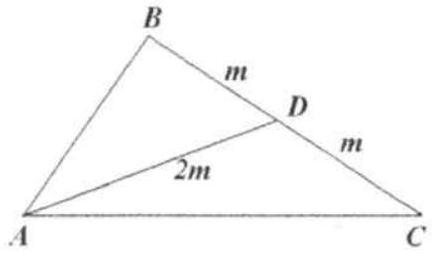
\includegraphics[width=\textwidth]{images/031(2).jpg}
\end{center}

\end{document}
